\begin{figure}[p]
\centering
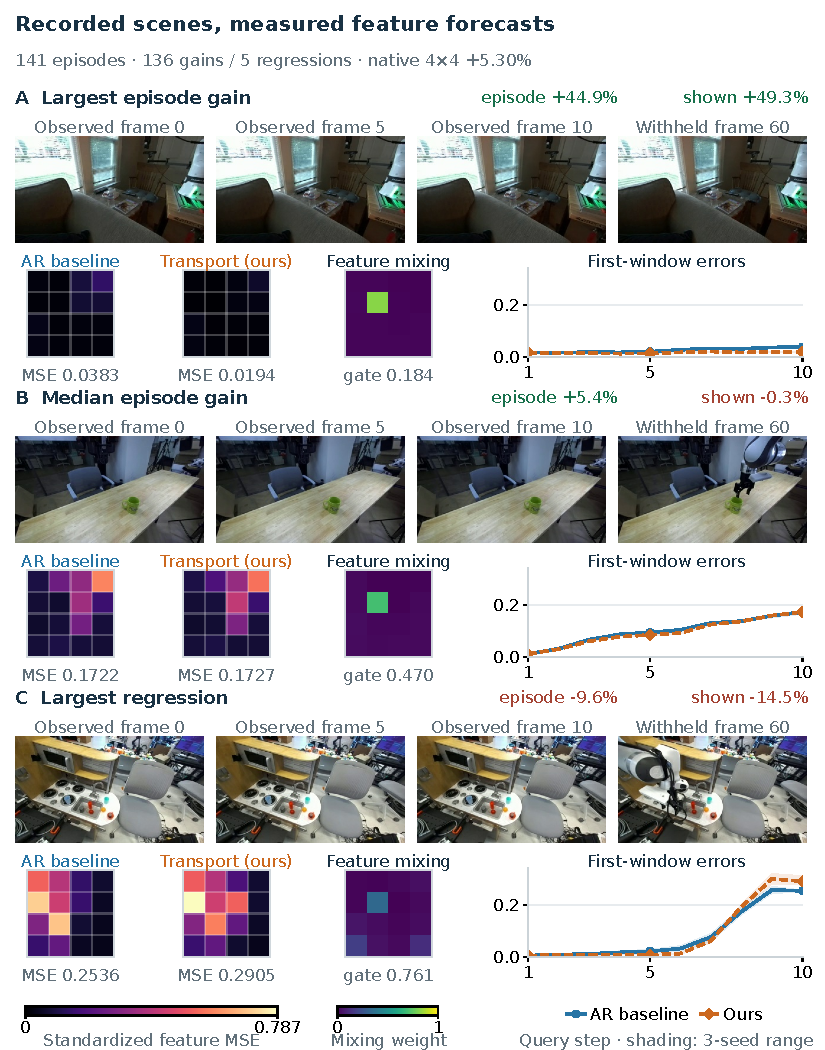
\includegraphics[width=\linewidth]{generated/real_video/spatial_qualitative.pdf}
\caption{\textbf{Recorded-video examples and spatial feature errors.} Best, median and worst cases use prespecified three-seed episode-level native h10 gain versus the matched $4\times4$ autoregressive baseline. The first eligible window is always shown: the median episode gains +5.358\%, but its displayed window regresses by -0.305\%. Withheld future frames enter only the evaluator. Images: DROID (CC BY 4.0). Error maps average squared standardized errors over 384 channels and three seeds, with one unclipped scale for all six maps. Curves show mean error and three-seed ranges (not confidence intervals): baseline, solid circles; ours, dashed diamonds. Mixing grids show actual h10 anchor-source weights for target cell (row 2, column 2), averaged across seeds; gates appear below. These are semantic feature mixtures, not physical flow or causal attribution. Population counts and episode- and seed-averaged native-grid endpoint gain appear above. This gain-conditioned validation gallery is not an independent test.}
\label{fig:spatial-qualitative}
\end{figure}
